% VUT FIT MITAI
% MSZ 2021/2022
% Author: Vladimir Dusek
% Login: xdusek27

%%%%%%%%%%%%%%%%%%%%%%%%%%%%%%%%%%%%%%%%%%%%%%%%%%%%%%%%%%%%%%%%%%%%%%%%%%%%%%%%

% Path to figures
\graphicspath{{msp/randomizovane_algoritmy/figures}}

%%%%%%%%%%%%%%%%%%%%%%%%%%%%%%%%%%%%%%%%%%%%%%%%%%%%%%%%%%%%%%%%%%%%%%%%%%%%%%%%

\chapter{MSP~--~Randomizované algoritmy (Monte Carlo a Las Vegas algoritmy).}

%%%%%%%%%%%%%%%%%%%%%%%%%%%%%%%%%%%%%%%%%%%%%%%%%%%%%%%%%%%%%%%%%%%%%%%%%%%%%%%%

\section{Zdroje}

\begin{compactitem}
    \item \path{MSP_13_Randomized_Algorithms.pdf}
    \item \path{MSP_2021-12-14_1080p.mp4}
\end{compactitem}

%%%%%%%%%%%%%%%%%%%%%%%%%%%%%%%%%%%%%%%%%%%%%%%%%%%%%%%%%%%%%%%%%%%%%%%%%%%%%%%%

\section{Úvod a kontext}

\begin{compactitem}
    \item K čemu jsou randomizované algoritmy? \begin{compactitem}
        \item Analyzujeme průměrné chování algoritmů (nikoliv nejhorší případ).

        \item Randomizací můžeme dosáhnout snížení očekávané ceny algoritmu.
    \end{compactitem}

    \item Přesahuje rámec analýzy nejlepšího nebo nejhoršího případu. \begin{compactitem}
        \item Analýza všech případů (vstupů) pomocí jejich pravděpodobnostního rozdělení.

        \item V mnoha případech poskytuje lepší vhled do praktické složitosti.

    \end{compactitem}

    \item Existují dva přístupy k randomizaci: \begin{compactitem}
        \item randomizace pořadí vstupů (např. Hiring Problem),

        \item randomizace volby provedené v rámci algoritmu (např. Quicksort).
    \end{compactitem}
\end{compactitem}

%%%%%%%%%%%%%%%%%%%%%%%%%%%%%%%%%%%%%%%%%%%%%%%%%%%%%%%%%%%%%%%%%%%%%%%%%%%%%%%%

\section{Indikátorová náhodná proměnná (\textit{indicator random variable})}

\begin{compactitem}
    \item Mějme prostor jevů $S$ a událost $A \in S$.

    \item Indikátorová náhodná proměnná pro $A$:
    $$ I\{A\} = \left\{
        \begin{array}{ll}
            1 & \text{pokud A nastane} \\
            0 & \text{jinak}
        \end{array}
        \right. $$

    \item Nechť $X_A = I\{A\}$, pak platí, že $E[X_A] = Pr\{A\}$ (pravděpodobnost výskytu události A).

    \item Hlavní myšlenka: Vyjádřit očekávání náhodné proměnné ($X$) jako očekávání sum komponent, které se snáze počítají (indikátorové proměnné $X_i$).
\end{compactitem}

\subsection{Příklad: Jaký je očekávaný počet padnutí orla při $n$ hodů mincí?}

$$ X_i = I\{ \text{i-tý hod mincí je událost padne orel} \}$$
$$ X = \sum_{i=1}^n X_i$$
$$ E[X] = E \left[ \sum_{i=1}^n X_i \right] = \sum_{i=1}^n E \left[ X_i \right] = \sum_{i=1}^n \frac{1}{2} = \frac{n}{2}$$

%%%%%%%%%%%%%%%%%%%%%%%%%%%%%%%%%%%%%%%%%%%%%%%%%%%%%%%%%%%%%%%%%%%%%%%%%%%%%%%%

\section{Hiring Problem}

\begin{compactitem}
    \item Firma chce nabrat nejlepšího zaměstnance.

    \item Můžeme randomizovat seznam kandidátů.

    \item Složitost ($c_h$ je cena najmutí nového kandidáta): \begin{compactitem}
        \item nejhorší případ: $\mathcal{O}(n \cdot c_h)$
        \item nejlepší případ: $\mathcal{O}(c_h)$
    \end{compactitem}

    \item Počet možných uspořádání kandidátů je $n!$, pak řešíme kolik permutací bude mít cenu $1, 2, \dots, n$.

\end{compactitem}

\begin{figure}[H]
    \centering
    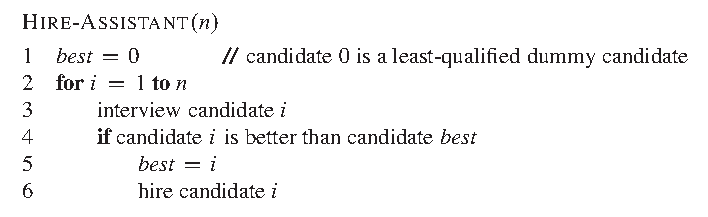
\includegraphics[width=0.8\linewidth]{hiring_problem.pdf}
    \caption{Hiring Problem v pseudokódu.}
\end{figure}

\begin{figure}[H]
    \centering
    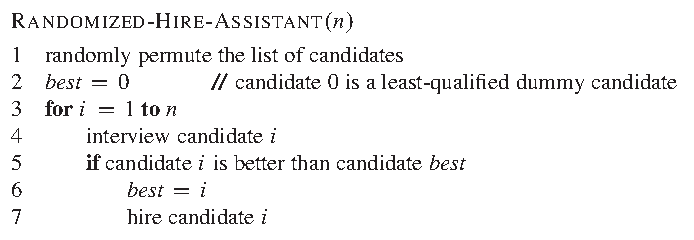
\includegraphics[width=0.8\linewidth]{hiring_problem_randomized.pdf}
    \caption{Hiring Problem randomizovaný v pseudokódu.}
\end{figure}

\subsection{Příklad: Analýza Hiring Problem pomocí indikátorové proměnné}

\begin{compactitem}
    \item Indikátorová proměnná.
    $$ X_i = I\{ \text{i-tý kandidát je přijat} \}$$

    \item Celkový počet přijatých kandidátů (cena).
    $$ X = \sum_{i=1}^n X_i$$

    \item Očekávaná cena algoritmu.
    $$ E[X] $$

    \item Pravděpodobnost, že i-tý kandidát je přijat (kandidát i je přijat, pokud je lepší, než všichni předchozí).
    $$ E[X_i] = \frac{1}{i}$$
    $$ E[X] = E \left[ \sum_{i=1}^n X_i \right] = \sum_{i=1}^n E \left[ X_i \right] = \sum_{i=1}^n \frac{1}{i} = \ln{n} + \mathcal{O}(1)$$

    \item Pravděpodobnostní analýza nám dává asymptotický lepší ohraničení ceny

    $$ \mathcal{O}(\log{n} \cdot c_h) ~~~\text{vs}~~~ \mathcal{O}(n \cdot c_h)$$
\end{compactitem}

%%%%%%%%%%%%%%%%%%%%%%%%%%%%%%%%%%%%%%%%%%%%%%%%%%%%%%%%%%%%%%%%%%%%%%%%%%%%%%%%

\section{Las Vegas}

\begin{compactitem}
    \item Pro každý vstup dává správné výsledky (korektnost je zaručena).

    \item Pro každý vstup existuje pravděpodobnost, že doba běhu bude delší než je žádoucí nebo očekávané.

    \item Analyzujeme čas běhu algoritmu, který odpovídá nějaké náhodné proměnné.
\end{compactitem}

\subsection{Příklad: Je dáno pole $A[1, 2, \dots, n]$ s $n$ prvky (kde $n$ je sudé). Polovina z prvků obsahuje nuly, druhá polovina obsahuje jedničky. Cíl: Najděte index který obsahuje jedničku. Zkonstruujte Las Vegas algoritmus.}

\bigskip\noindent\begin{minipage}{\linewidth}
    \begin{lstlisting}[language=Python, caption={Las Vegas algoritmus v Pythonu.}]
def las_vegas(A, n):
    while True:
        i = random_int(0, n)
        if A[i] == 1:
            return i
\end{lstlisting}
\end{minipage}

\begin{compactitem}
    \item Průměrná složitost je $\mathcal{O}(1)$, to můžeme ukázat pomocí očekávané doby běhu s využitím indikátorové proměnné:
    $$ X_i = \left\{
        \begin{array}{ll}
            1 & \text{pokud algoritmus provede i-té porovnání} \\
            0 & \text{jinak}
        \end{array}
        \right. $$
    $$ X = \sum_{i=1}^{\infty} X_i $$
    $$ E[X] = E \left[ \sum_{i=1}^{\infty} X_i \right] = \sum_{i=1}^{\infty} E \left[ X_i \right] = \sum_{i=1}^{\infty} Pr\{ X_i \} =\sum_{i=1}^{\infty} \left(\frac{1}{2}\right)^{i-1} = 2 = \mathcal{O}(1)$$
\end{compactitem}

\subsection{Příklad: Analýza Quicksortu.}

\begin{compactitem}
    \item Myšlenka randomizace: výběr pivota.
\end{compactitem}

\noindent\begin{minipage}{\linewidth}
    \begin{lstlisting}[language=Python, caption={Quicksort v Pythonu.}]
def quicksort(numbers: list[int]) -> list[int]:
    if not numbers:
        return []
    pivot = get_random_elem(numbers)
    less = []
    greater = []
    for number in numbers:
        if number < pivot:
            less.append(number)
        elif number > pivot:
            greater.append(number)
    return [*quicksort(less), pivot, *quicksort(greater)]
\end{lstlisting}
\end{minipage}

\begin{compactitem}
    \item V nejhorším případě: $\mathcal{O}(n^2)$. \begin{compactitem}
        \item Pivotem je zvoleno vždy největší nebo nejmenší číslo.
    \end{compactitem}

    \item V nejlepším případě: $\mathcal{O}(n \cdot \log{n})$. \begin{compactitem}
        \item Pivotem je zvoleno vždy číslo uprostřed.
    \end{compactitem}

    \item Průměrný případ pomocí pravděpodobnostní analýzy: \begin{compactitem}
        \item Sestrojení indikátorové proměnné. Vyjadřuje, zda dvojice prvků spolu byla porovnána.
        $$ X_{ij} = \left\{
            \begin{array}{ll}
                1 & \text{pokud } x_i \text{ a } x_j \text{spolu byly porovnány} \\
                0 & \text{jinak}
            \end{array}
            \right. $$

        \item Celkový počet porovnání:
        $$ X = \sum_{1 \leq i \leq j \leq n} X_{ij} $$
        $$ E[X] = \sum_{1 \leq i \leq j \leq n} Pr[x_i \text{ a } x_j \text{ jsou porovnány}] $$

        \item Nechť $y_1, y_2, \dots, y_n$ jsou vstupní prvky v seřazeném pořadí (suma je komutativní, takže lze provést).
        $$ E[X] = \sum_{1 \leq i \leq j \leq n} Pr[y_i \text{ a } y_j \text{ jsou porovnány}] $$

        \item \textit{Pro výpočet viz přednášku, je to nad rámec a nebude se zkoušet.}
        $$ Pr[y_i \text{ a } y_j \text{ jsou porovnány}] = \frac{2}{j - i + 1} $$
        $$ E[X] = \sum_{1 \leq i \leq j \leq n} \frac{2}{j - i + 1} = \ldots = 2n \cdot \ln{n} = \mathcal{O}(n \cdot \log{n})$$

    \end{compactitem}
\end{compactitem}

%%%%%%%%%%%%%%%%%%%%%%%%%%%%%%%%%%%%%%%%%%%%%%%%%%%%%%%%%%%%%%%%%%%%%%%%%%%%%%%%

\section{Monte Carlo}

\begin{compactitem}
    \item Pro každý vstup existuje pravděpodobnost výskytu chyby (nesprávného výsledku).

    \item Je zaručena doba běhu algoritmu.

    \item Pro maximalizaci korektnosti využívá tzv. aplifikaci -- pokud algoritmus neskončí korektně, tak se opakuje, opakování je zastropováno konstantou. \begin{compactitem}
        \item Myšlenka: mám algoritmus kterej je v podstatě k ničemu (je velmi malá šance, že je korektní), ale hodněkrát ho opakuju.
    \end{compactitem}

    \item Analyzujeme čas běhu a pravděpodobnost korektnosti algoritmu.
\end{compactitem}

\subsection{Příklad: Je dáno pole $A[1, 2, \dots, n]$ s $n$ prvky (kde $n$ je sudé). Polovina z prvků obsahuje nuly, druhá polovina obsahuje jedničky. Cíl: Najděte index který obsahuje jedničku. Zkonstruujte Monte Carlo algoritmus.}

\bigskip\noindent\begin{minipage}{\linewidth}
    \begin{lstlisting}[language=Python, caption={Monte Carlo algoritmus.}]
def monte_carlo(A, n):
    limit = 1000
    for _ in range(0, limit):
        i = random_int(0, n)
        if A[i] == 1:
            return i
    return None
\end{lstlisting}
\end{minipage}

\begin{compactitem}
    \item Složitost: $\mathcal{O}(1)$.
    \item Pravděpodobnost korektnosti: $1 - 0,5^{1000} $
\end{compactitem}

\subsection{Příklad: Problém minimálního řezu v grafu}

\begin{compactitem}
    \item Problém minimálního řezu v grafu (\textit{min cut problem}) spočívá v rozdělení množiny uzlů na dvě neprázdné podmnožiny takovým způsobem, že počet hran, které vedou z jedné podmnožiny do druhé je minimální.

    \item Myšlenka randomizace: náhodně slučujeme vrcholy.
\end{compactitem}

\begin{figure}[H]
    \centering
    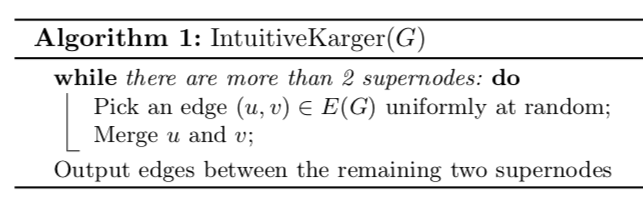
\includegraphics[width=0.75\linewidth]{min_cut_alg.png}
    \caption{Algoritmus v pseudokódu.}
\end{figure}

\begin{figure}[H]
    \centering
    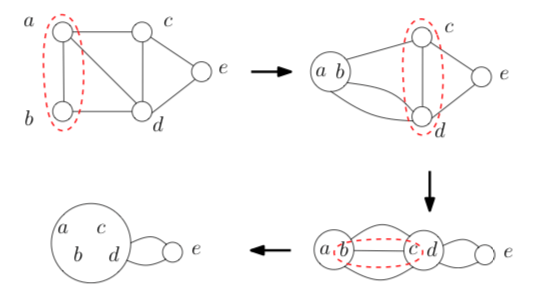
\includegraphics[width=0.75\linewidth]{min_cut_visualizaiton.png}
    \caption{Algoritmus vizualizace.}
\end{figure}

\begin{compactitem}
    \item Algoritmus má garantovanou složitost $\mathcal{O}(n^2)$ -- každé sloučení stojí $\mathcal{O}(n)$.

    \item Šance, že algoritmus je v tomto stavu korektní, je velmi malá $\Theta(\frac{1}{n^2})$, proto je nutné zavést amplifikaci. \begin{compactitem}
        \item Zavedeme konstantu $c$ a algoritmus poběží:
        $$c \cdot n^2 \cdot \ln{n}$$
        \item Složitost:
        $$\mathcal{O}(n^4 \log{n})$$
        \item Pravděpodobnost korektního běhu pak je:
        $$1 - \frac{1}{n^c}$$
    \end{compactitem}

    \item Reálné použití spočívá typicky v kombinaci randomizace a \textit{brute force} přístupu. Na začátku randomizujeme, protože je menší šance, že bude porušena korektnost. Tím se problém redukujeme na menší (v případě min-cut se graf zmenšuje). Čím menší instance problému, tím je vyšší pravděpodobnost porušení korektnosti, ale zároveň se cena \textit{brute force} řešení snižuje. Tedy, až je instance problému dostatečně malá (graf je dostatečně malý), tak provedeme jeho vyřešení \textit{brute force} algoritmem (který je korektní).
\end{compactitem}
